\documentclass[12pt,a4paper]{report}	
\usepackage[utf8]{inputenc}
\usepackage{textcomp}
\usepackage{amsmath}
\usepackage{amsfonts}
\usepackage{amssymb}
\usepackage{color}
\usepackage{graphicx}
\usepackage{lscape}						%Landscape enabled. Doh!
\usepackage{longtable}					%To set table as multi-page
\usepackage{anysize}					%To set margins below
\marginsize{2cm}{2cm}{1cm}{3cm} 		%left, right, top, bot margin
\usepackage{float}						%Control table float
\usepackage{standalone}					%Clear formatting in other documents included
\usepackage{color}						%This and next for the \hilight keyword. 
\newcommand{\hilight}[1]{\colorbox{yellow}{#1}}

\setcounter{secnumdepth}{3} %To get nummerated \subsubsection{title}
\setcounter{tocdepth}{3}	%To get nummerated \subsubsection{title}

\begin{document}
\chapter{Timeboxes}
Of cause all teammembers will help eachother and discuss the different elements throughout the project, but the members of the team must choose a topic to specialize in. Below a short description is made to divide the members into groups of specialization, acting as guidelines for who is in charge of the development in the different areas:
\begin{itemize}
\item \textbf{Morten - Software} in charge of C/C++ and Linux programming, in cooperation with Henrik.
\item \textbf{Henrik - Software specialization} with most experience in C/C++ algorithms be cooperating with Morten.
\item \textbf{Jacob - DSP and Analog specialization} will be in charge of the DSP and Analog area, in cooperation with Anders.
\item \textbf{Anders - FPGA and DSP specialization} will cooperate together with Jacob in implementing and computing the elements containing DSP, Analog technique and FPGA design.
\end{itemize}
This is just as guidelines, everyone will of cause have knowledge about the elements the other team members are developing.


\documentclass[12pt,a4paper]{report}	
\usepackage[utf8]{inputenc}
\usepackage{textcomp}
\usepackage{amsmath}
\usepackage{amsfonts}
\usepackage{amssymb}
\usepackage{color}
\usepackage{graphicx}
\usepackage{lscape}						%Landscape enabled. Doh!
\usepackage{longtable}					%To set table as multi-page
\usepackage{anysize}					%To set margins below
\marginsize{2cm}{2cm}{1cm}{3cm} 		%left, right, top, bot margin
\usepackage{float}						%Control table float

\setcounter{secnumdepth}{3} %To get nummerated \subsubsection{title}
\setcounter{tocdepth}{3}	%To get nummerated \subsubsection{title}

\begin{document}
\section{Timebox 1}

\subsection{Outline for this timebox}
\begin{enumerate}
\item Module design of entire system. (Detailed)
\item Design CpuInterface, for communication between FPGA and LPC.
\item Implement CpuInterface.
\end{enumerate}

\subsection{Development Plan}


\subsection{Results}

\subsubsection{Module Design (Jacob)} 
\paragraph{Requirements to fulfil}\mbox{}\\
4.a\\

\begin{itemize}
	\item Each team shall write a small module design, before implementation.
	\begin{itemize}
		\item The module design shall be approved during timebox-deployment, BEFORE implementation begins.
	\end{itemize}
\end{itemize}


\paragraph{Theory}\mbox{}\\
The module design shall help us clarify which blocks shall be implemented where. All the hardware, the Spartan 3A board, the LPC2478 and other modules, shall be drawn an connected. This clarifies what the different hardware contains and how they interface with each other. The module design is shown in Figure \ref{fig:module_design_v0_9}

\begin{landscape}
\begin{figure}[h!]
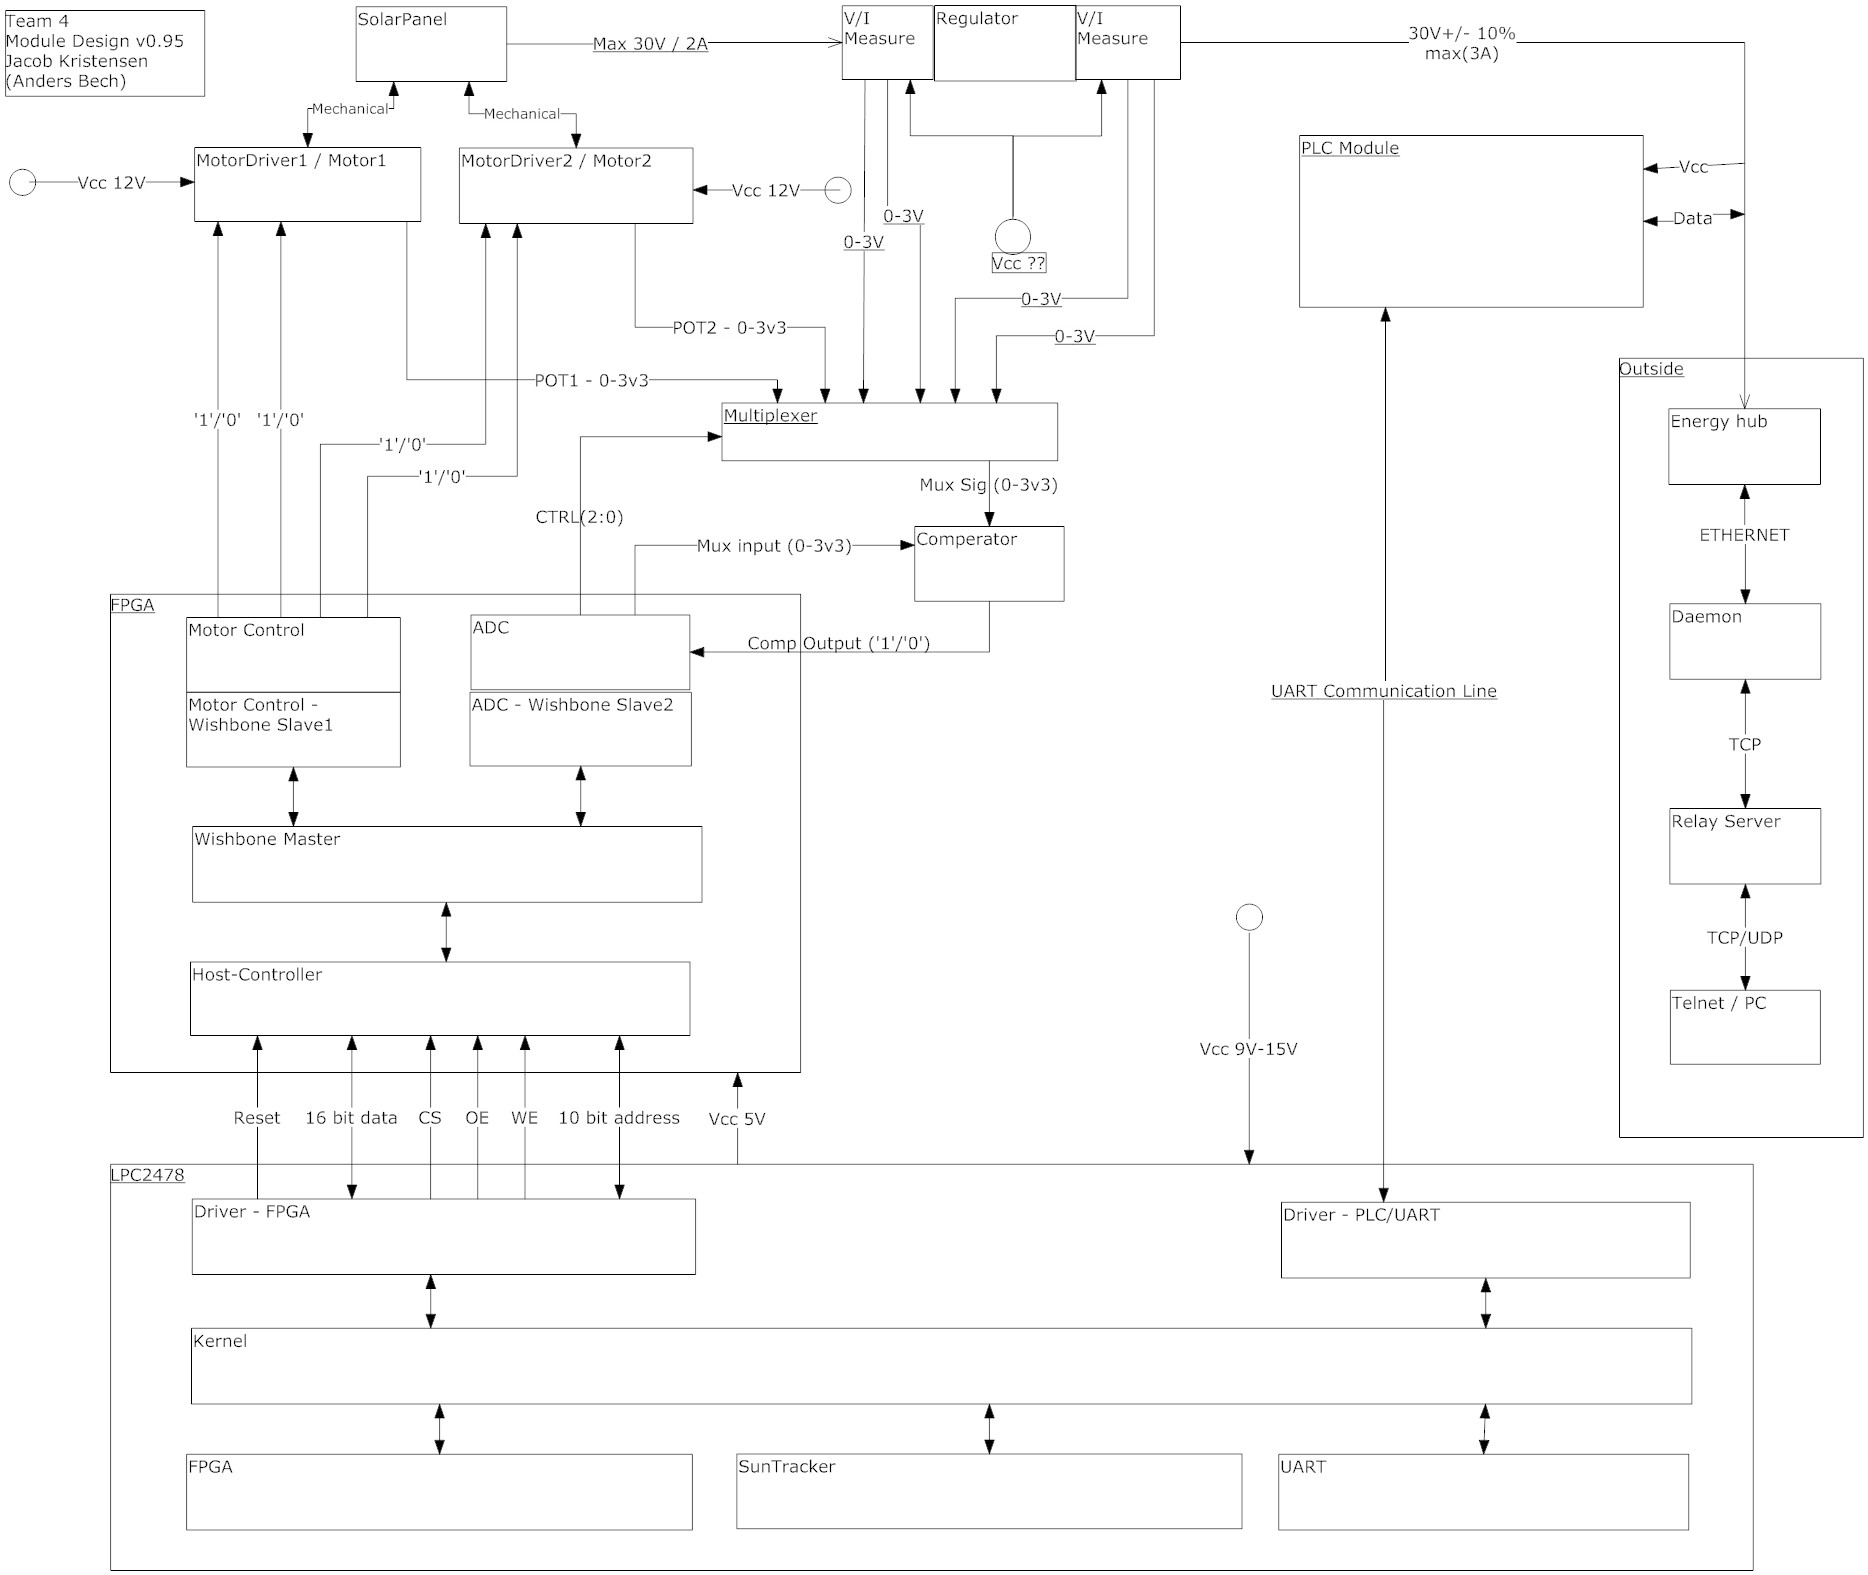
\includegraphics[width=20CM]{./img/module_design_v0_9_5}
\caption{Module Design of "system-to-be"}
\label{fig:module_design_v0_9}
\end{figure}
\end{landscape}

The \textbf{solar panel} is physically connected to the two motors, which will turn the panel towards the sun. \textbf{The two motors} are each supplied by 12 V DC (Source unknown). Four signals are received from the \textbf{FPGA}, that controls which way the motors have to turn. Those signals are sent to two H-bridges, which will invert the voltage, and make the motors turn in different directions. The four signals are controlled by a \textbf{PWM} block in the FPGA, to make speed control of the motors possible. \\
The potentiometers of the motors will return a value to the \textbf{ADC} implemented in the FPGA, which then can compare their position, to the position of the sun, received from the LPC2478. The ADC input limit, on the FPGA board is 3v3\footnote{FPGA datasheet page 3.}\\
The ADC and the PWM are implemented in a wishbone structure, which makes it possible to use it at different platforms, if the wishbone interfaces are obeyed. The two wishbone slaved (PWM, ADC), are interfaced to the LPC2478 through a wishbone master, controlling the communication, and then through a host-controller, onto the FPGA-driver implemented on the LPC2478 board. \\
The SPARTAN 3A board and the LPC2478 developers kit is a requirement to this project, given by the teachers. The \textbf{FPGA} board is software coded hardware, which means it makes most sense to replace some actual hardware by this development board, or maybe make a module more efficient, by replacing some of the software by this "hardware" board. In this case it is replaced by both. The suntracker was meant as pure software, but now a formula, calculating the position of the sun, is implemented as software, and the position of the sun is sent to the FPGA; which compares it to the position of the motors, received by the potentiometers, and then repositioning the motors, according to the sun. \\
The \textbf{LPC2478} board is where the software is placed, and are an essential part of the system. This is used for communication, logging and other things, which will be described later. The board is controlled by a small embedded Linux system. Three drivers are implemented, and they are controlled by the kernel, on behalf of three user applications. This board is supplied with a voltage between 9-15V DC\footnote{LPC2478 print}. \\
The first interface was the interface for communication with the FPGA, shortly described above. This is a 16 bit communication line, which is also a requirement for the system. Further there is a chip select, read and write line and finally a supply line, supplying the FPGA with power from the LPC2478 board\footnote{LPC2475 user manual, chap. 5 - External Memory Controller}. The FPGA user application will handle the information that is to be sent and received. \\
The power generated from the solar panel, will be sent through a \textbf{regulator}, which is pure hardware, where the power will be converted from approx 30V, into 30V+/-10\%. This output is a common requirement, to make the system function with the other systems. \\
Two galvanic isolated \textbf{sensors} are applied to the input and the output of the regulator, to keep track of how much energy is produced and how efficient the regulator is. Those sensors sends a PWM signal (0-3v)\footnote{LPC2478 user manual, chap 28.2} down to the ADC, in the sensor driver, in the LPC2478 board. The user application to the sensor driver will then pack the data and send them to the energy hub, which updates the web-page. \\
The last user application/driver at the LPC board is the \textbf{PLC driver}, which makes the communication to the energy hub possible. This communication is established through UART, which sends and receives messages between the system and the energy-hub. A\textbf{ PLC module} is implemented too, which is supplied by the powerline and speaks through it too. 

\paragraph{verification of requirements}\mbox{}\\








% %Wishbone interface

\subsubsection{Implementation of the wishbone interface (Jacob)} 
\paragraph{Requirements to fulfil}  \mbox{}\\
FR.3.b.i\\
\textit{Capable of decoding 16 bit read and write from the LPC2478.}\\
This requirement will not be entirely fulfilled in this timebox, but it has to be taken into account, because the CpuInterface, that has to be implemented in this timebox, shall be capable of communicating through a 16 bit data bus, with the LPC2478.\\
NR.4.b\\
\textit{Your VHDL design shall be implemented in following files:
	\begin{itemize}
		\item name.vhd containing the RTL implementation.
		\item tb\_name.vhd containing a testbench for your module(s) above.
		\item name.uch containing the user constrains for your FPGA implementation.
	\end{itemize}}

\paragraph{Theory}\mbox{}

\subparagraph{Pin Budget}
There is a limited amount of GPIO pins available at the FPGA board, so a detailed pin budget will be made, to clarify how many pins are needed and which function each pin will have. This is essential to design the modules inside the FPGA, or at least to make them work prober without much confusion.


\begin{figure}[H]
\centering
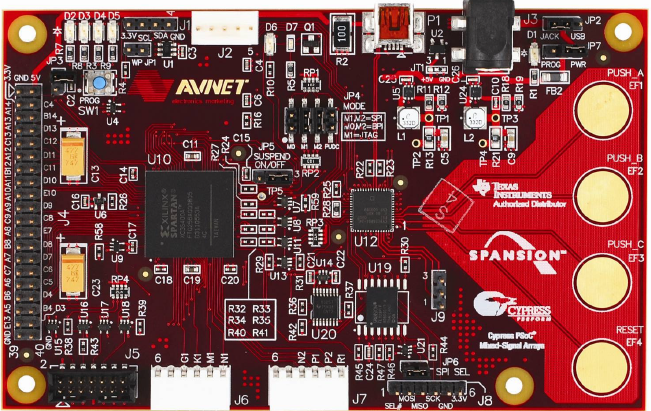
\includegraphics[width=\textwidth]{./img/Spartan3Aboard}
\caption{Spartan 3A board}
\label{fig:Spartan3Aboard}
\end{figure}




Figure \ref{fig:Spartan3Aboard} shows the layout of the Spartan 3A board. The pin connectors J4, J6 and J7 will be used. For the CPU interface, only J4 will be used. 

%DATA
\begin{table}[H]
\begin{center}
\caption{Data Pins}
\begin{tabular}{|l|l||l|l||l|}
\hline FPGA & FPGA & LPC & LPC & FUNCTION \\ 
PIN \# & PIN & PIN\# & PIN & \\
 & NAME &  & NAME & \\
\hline J4 4 & C4 & J2 60 & BD0 & DATA\_PIN0 \\ 
\hline J4 5 & A14 & J2 58 & BD2 & DATA\_PIN2 \\ 
\hline J4 6 & B14 & J2 56 & BD4 & DATA\_PIN4 \\ 
\hline J4 7 & A13 & J2 54 & BD6 & DATA\_PIN6 \\ 
\hline J4 8 & D13 & J2 52 & BD8 & DATA\_PIN8 \\ 
\hline J4 9 & C13 & J2 50 & BD10 & DATA\_PIN10 \\ 
\hline J4 10 & C12 & J2 48 & BD12 & DATA\_PIN12 \\ 
\hline J4 11 & A12 & J2 46 & BD14 & DATA\_PIN14 \\ 
\hline J4 12 & D11 & J2 59 & BD1 & DATA\_PIN1 \\ 
\hline J4 13 & B12 & J2 57 & BD3 & DATA\_PIN3 \\ 
\hline J4 14 & C11 & J2 55 & BD5 & DATA\_PIN5 \\ 
\hline J4 15 & A11 & J2 53 & BD7 & DATA\_PIN7 \\ 
\hline J4 16 & D10 & J2 51 & BD9 & DATA\_PIN9 \\ 
\hline J4 17 & A10 & J2 49 & BD11 & DATA\_PIN11 \\ 
\hline J4 18 & E10 & J2 47 & BD13 & DATA\_PIN13 \\ 
\hline J4 19 & A9 & J2 45 & BD15 & DATA\_PIN15 \\ 
\hline 
\end{tabular} 
\label{table:datatab} %\ref{table:datatab}
\end{center}
\end{table}

Table \ref{table:datatab} shows the data pins connections. Referring to  FR 3.a.i \& FR 3.b.i, 16 pins are reserved for the data transfer. 


%ADRESS
\begin{table}[H]
\begin{center}
\caption{Adress Pins}
\begin{tabular}{|l|l||l|l||l|}
\hline FPGA & FPGA & LPC & LPC & FUNCTION \\ 
PIN \# & PIN & PIN\# & PIN & \\
 & NAME &  & NAME & \\
\hline J4 20 & D9 & J2 42 & BA0 & ADDR\_PIN0 \\ 
\hline J4 21 & C9 & J2 40 & BA2 & ADDR\_PIN2 \\ 
\hline J4 22 & C8 & J2 38 & BA4 & ADDR\_PIN4 \\ 
\hline J4 23 & A8 & J2 36 & BA6 & ADDR\_PIN6 \\ 
\hline J4 24 & E7 & J2 34 & BA8 & ADDR\_PIN8 \\ 
\hline J4 25 & B8 & J2 41 & BA1 & ADDR\_PIN1 \\ 
\hline J4 26 & D8 & J2 39 & BA3 & ADDR\_PIN3 \\ 
\hline J4 27 & A7 & J2 37 & BA5 & ADDR\_PIN5 \\ 
\hline J4 28 & D7 & J2 35 & BA7 & ADDR\_PIN7 \\ 
\hline J4 29 & C7 & J2 33 & BA9 & ADDR\_PIN9 \\ 
\hline 
\end{tabular} 
\label{table:addrtab} %\ref{table:addrtab}
\end{center}
\end{table}

Table \ref{table:addrtab} shows the address pins used. 10 pins are reserved for address. 


\begin{table}[H]
\begin{center}
\caption{Motor Control Pins}
%MOTOR CONTROL
\begin{tabular}{|l|l||l|}
\hline FPGA & FPGA &  FUNCTION \\ 
PIN \# & PIN & \\
 & NAME & \\
\hline J4 31 & A6 & M\_CTRL4 \\ 
\hline J4 32 & C5 & M\_CTRL3 \\ 
\hline J4 33 & B6 & M\_CTRL2 \\ 
\hline J4 34 & D4 & M\_CTRL1 \\ 
\hline 
\end{tabular} 
\label{table:mctrltab} %\ref{table:mctrltab}
\end{center}
\end{table}

Table \ref{table:mctrltab} shows the four pins reserved for motor control. 4 output signals to two H-bridges, to control the motors position. One pin for each direction the solar panel has to move; up, down, left right. 


\begin{table}[H]
\begin{center}
\caption{LPC/FPGA Control Pins}
%LPC/FPGA CONTROL
\begin{tabular}{|l|l||l|l||l|}
\hline FPGA & FPGA & LPC & LPC & FUNCTION \\ 
PIN \# & PIN & PIN\# & PIN & \\
 & NAME &  & NAME & \\
\hline J4 35 & A5 & J1 45 & 2.14 & Chip Select \\ 
\hline J4 36 & B4 & J1 6 & Reset\_out & Reset \\ 
\hline J4 37 & E13 & J1 35 & BWE & Write Enable \\ 
\hline J4 38 & D3 & J1 36 & BOE & Output Enable \\ 
\hline 
\end{tabular} 
\label{table:lpctab} %\ref{table:lpctab}
\end{center}
\end{table}

Table \ref{table:lpctab} shows the chip select, which has to be high for the FPGA to react on commands from the LPC, Reset for a synchronous reset of both boards. When reset is pressed on the LPC board, Reset\_out will be set low, which the FPGA will react on. Also if the power is lost, the pin will go low, and secure a reset/idle state, until the power is turned on again. Also the Write and Read enable are described, for the LPC to control whether the FPGA has to send or receive data from the LPC. 


\begin{table}[H]
\begin{center}
\caption{LPC Control Pins}
%LPC/FPGA CONTROL
\begin{tabular}{|l||l|l||l|}
\hline  Connection 	& LPC 	& LPC 	& FUNCTION \\ 
 	 				& PIN\# & PIN 	& \\
 	 				&  		& NAME 	& \\
\hline  Chip Select	& J2 43 & DBUS\_EN & Data Bus Enable \\
\hline  Ground		& J2 44 & ABUF\_EN & Address Buffer Enable \\
\hline 
\end{tabular} 
\label{table:bustab} %\ref{table:bustab}
\end{center}
\end{table}

Table \ref{table:bustab} shows that DBUS\_EN is connected to Chip Select. This is enabled when chip select is enabled. This data bus is controlled by the WE and OE signals, and can act both as input and output. This should not be left low, else it will collide with the boards internal data bus, therefore it is connected to Chip Select, and is only low when chip select is enabled. DBUS\_EN is active low. \\
ABUF\_EN is grounded, to pull it low constantly. This will enable the two buffers for address. Also the control signals are enabled, and act as output. \footnote{LPC2478\_OEM\_Board\_Users\_Guide\_Rev\_H, page 10, chap 3.1.6}


\begin{table}[H]
\begin{center}
\caption{Others}
%OTHERS
\begin{tabular}{|l|l||l|}
\hline FPGA & FPGA & FUNCTION \\ 
PIN \# & PIN & \\
 & NAME & \\
\hline J4 1 & GND & GND \\ 
\hline J4 2 & +5V & +5V SUPPLY \\ 
\hline J4 3 & +3.3V & +3.3 SUPPLY \\ 
\hline J4 30 & C6 & FREE \\ 
\hline J4 39 & GND & GND \\ 
\hline J4 40 & GND & GND \\ 
\hline 
\end{tabular} 
\label{table:otherstab} %Uset to refer to table: \ref{table:otherstab}
\end{center}
\end{table}
A lot of text, to describe the table of data!

\subparagraph{State Machine Diagram (Jacob)}
Before implementing the VHDL code, a state machine diagram is made to clarify which states the module has to go through. When this is in place, the code is very easy to implement.
\begin{figure}[H]
\centering
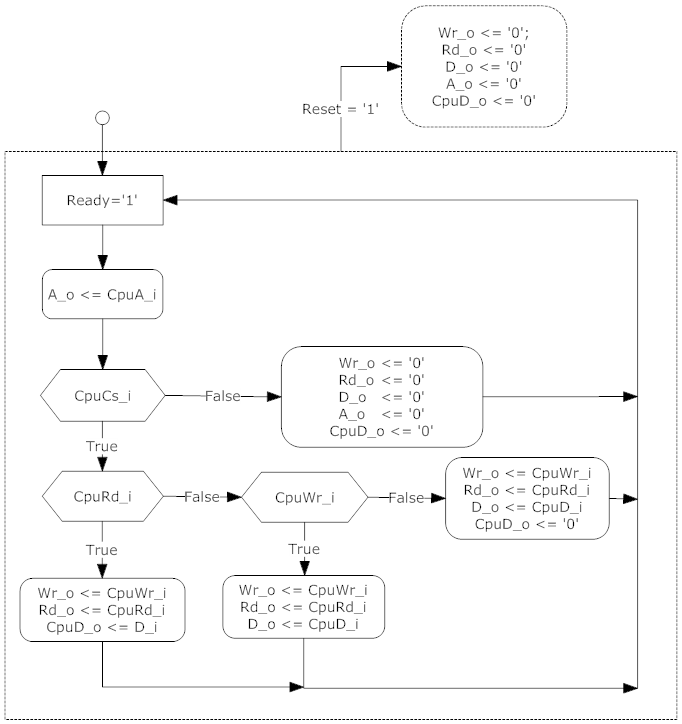
\includegraphics[width=10cm]{./img/State_Machine_Diagram_CpuInterface_v0_9}
\caption{State Machine Diagram - CpuInterface}
\label{fig:State_Machine_Diagram_CpuInterface_v0_9}
\end{figure}
Figure \ref{fig:State_Machine_Diagram_CpuInterface_v0_9} shows the State MAchine Diagram for the CpuInterface. The different states will be discussed in the "implementation" chapter below.

\paragraph{Implementation}\mbox{}\\
Important thing first. The module has to check if the reset pin is enabled. If this is the case, it has to reset the board, no matter what. This is why it is set asynchronious. No clock has to be on its rising or falling edge. The reset values is all 0, to be sure no data is stored, no adress is stored and no write/read commands are given to the Wishbone Master. 
\begin{verbatim}
-- Check if reset=high (Unsynchronized)

	-- Reset all values to '0'

	if(Rst='1') then

		Wr_o <= '0';

		Rd_o <= '0';

		D_o <= (others => '0');

		A_o <= (others => '0');

		CpuD_o <= (others => '0');
\end{verbatim}

If reset is not set, the module has to think syncronous. This is why we check the clock. Both the read and write state is inside the synchronous clock state, and also the chip select (CpuCs\_i) has to be high, in order for the module to respond on read/write commands. When chip select is set high, the adress is sent from the Cpu to the Wishbone Master. The adress can always be set, without any failures occur.\\
Then it is time to check if the "Read" is set. If it is, then the CPU wants to read data from the FPGA, thats why the data from the Wishbone master (D\_i) is sent to the output to the cpu (CpuD\_o).\\
Also the Read and Write input from the cpu is sent to the wishbone master. Then the cpu will have to avoid both being high at the same time. 
\begin{verbatim}
	elsif(Clk'event and Clk = '1') then --(All sync)	

	-- Check if active read (CPU read ffrom FPGA)

		if(CpuCs_i = '1') then

		A_o <= CpuA_i; -- Common for all

			if(CpuRd_i = '1') then

				Wr_o <= CpuWr_i; 	-- Enables/Disables master write

				Rd_o <= CpuRd_i; 	-- Enables/Disables master read

				CpuD_o <= D_i;		-- Data from master (D_i) to CPU (CpuD_o)
\end{verbatim}

If read is not high, the write pin has to be checked. If that is enabled, the CpuInterface will send the data recieved from the Cpu to the Wishbone master. Again both read and write is rooted directly to the Wishbone Master.
\begin{verbatim}
			-- Check if active write (CPU write to FPGA)

			elsif(CpuWr_i = '1') then

				Wr_o <= CpuWr_i;	

				Rd_o <= CpuRd_i;

				D_o <= CpuD_i;		-- Data from CPU (CpuD_i) to Master (D_o)

			else
\end{verbatim}


If either read nor write is high, the Cpuinterface will reset the Cpu data out to all "0". Also the read and write are directly rooted to the wishbone master, which also is "0". This will keep the system from making any action when not supposed to. 
\begin{verbatim}
			-- Reset values to 0

				Wr_o <= CpuWr_i;

				Rd_o <= CpuRd_i;

				D_o <= CpuD_i;

				CpuD_o <= (others => '0');

			end if;
\end{verbatim}

Last but not least, if chip select is not enabled, all values will be reset, as iff the reset button was pressed. This is to avoid any failures and unwanted actions in the system. 
\begin{verbatim}
		-- If Chip not selected (CpuCs_i = '0'), reset all values to '0'.

		else 

			Wr_o	<= '0';

			Rd_o 	<= '0';

			D_o	<= (others => '0');

			A_o	<= (others => '0');

			CpuD_o <= (others => '0');

		end if;

	end if;
	end process Cpuinter;
\end{verbatim}

\paragraph{verification}\mbox{}\\

By inspecting the VHDL code for the CpuInterface,i find the names correct.\\
\begin{centering}

cpuinterface.vhd\\
Avnet\_Sp3A\_Eval\_081201.ucf\\
tb\_Cpuinterface.vhd

\end{centering}
By running the testbench, it can be found out, if the behaviour og the Cpuinterface is correct. Figure \ref{fig:tb_CpuInterface} shws a screenshot of the testbench. 
\begin{figure}[htbp]
\centering
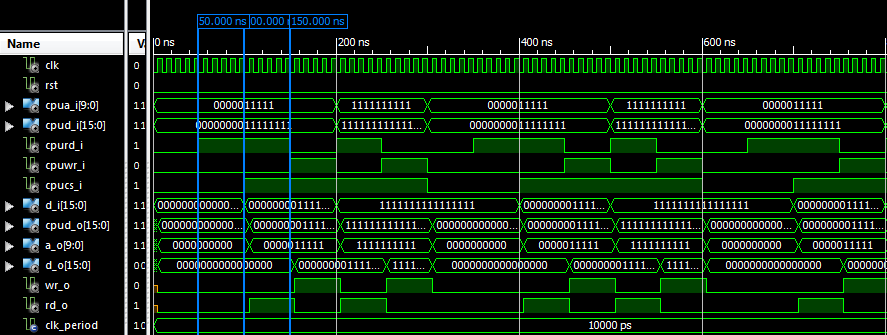
\includegraphics[width=\textwidth]{./img/tb_CpuInterface}
\caption{Testbench - CpuInterface}
\label{fig:tb_CpuInterface}
\end{figure}

At the first blue marker, the rd\_i is set high, but no data is read from the FPGA. This is right, because the Chip Select is NOT high. At the second marker, this is set high, and the data is read. The third marker shows the rd\_i going low, and the Wr\_i going high. Here the data is written to the FPGA. This confirms that the Cpuinterface works as it is supposed to. 




\end{document}





\documentclass[12pt,a4paper]{report}	
\usepackage[utf8]{inputenc}
\usepackage{textcomp}
\usepackage{amsmath}
\usepackage{amsfonts}
\usepackage{amssymb}
\usepackage{color}
\usepackage{graphicx}
\usepackage{lscape}						%Landscape enabled. Doh!
\usepackage{longtable}					%To set table as multi-page
\usepackage{anysize}					%To set margins below
\marginsize{2cm}{2cm}{1cm}{3cm} 		%left, right, top, bot margin
\usepackage{float}						%Control table float

\setcounter{secnumdepth}{3} %To get nummerated \subsubsection{title}
\setcounter{tocdepth}{3}	%To get nummerated \subsubsection{title}

\begin{document}
\section{Timebox 2}
\subsection{Outline for this timebox}
This timebox includes a project week and a Easter holiday, week 13 \& 14.
\begin{enumerate}
\item Get information about the effect of the Photo Voltaic.
\item Implement the wishbone interface (Jacob)
\item Design VHDL diagram for Slave 1 (Anders (Jacob))
\item Design VHDL diagram for Slave 2 (Anders (Jacob))
\item Design software for SunTracker (Morten \& Henrik)
\item Implement software for SunTracker (Morten \& Henrik)
\item Design Voltage Measure PCB for logger (Jacob)
\item Design Current Measure PCB for logger (Jacob)
\item Design Software for Communicator (Henrik)
\end{enumerate}

\subsection{Development Plan}


\subsection{Results}


\subsubsection{Design \& implement code for SunTracker (Morten \& Henrik)}
\paragraph{Requirements to fulfil}\mbox{}\\
FR 1.a\\
FR 1.c

\paragraph{Theory}\mbox{}\\
The SunTracker function will be operated by the system calling it with 3 variables that can be obtained through the RTC, a fail safe has been made so the system will only access the rest of the code if 4 argument counts has been given.
\begin{verbatim}
int main(int argc, char *argv[]) {
	int hr;
	int min;
	int day;
	if (argc != 4) {
		printf("Usage: [hr] [min] [date int]");
		exit(1);

	}
\end{verbatim}

meaning that if the system hasn't send the 4 arguments then the code will write back to the user that he has to send the arguments in order hour - minutes - date int in order to get the sun position corresponding to the time sent.

\paragraph{Implementation}\mbox{}\\
A Makefile is made in order to convert the file type to a hex file that can run in the user space on uClinux on the LPC2478 board. 
\begin{verbatim}
EXEC = SolarPosition
   OBJS = SolarPosition.o sunpos.o
 
   all: $(EXEC)
 
   $(EXEC): $(OBJS)
	arm-elf-gcc $(LDFLAGS) -o $@ $(OBJS) $(LDLIBS) -elf2flt -lm

SolarPosition.o : SolarPosition.c sunpos.h 
	arm-elf-gcc -c SolarPosition.c
 
sunpos.o : sunpos.c sunpos.h
	arm-elf-gcc -c sunpos.c

   romfs:
	$(ROMFSINST)    /bin/$(EXEC)
 
   clean:
	rm -f $(EXEC) *.elf *.gdb *.o
\end{verbatim}

The executeable file that will be made is called "SolarPosition" it is composed of two object files called SolarPosition.o and Sunpos.o which in turn are composed by a header file called sunpos.h and a c file called the same as the object file itself.
a command to clean the files made by the Makefile is also made, it will clean the executeable file itself, and all elf, gdb and object files. 
after the executeable file it made, then it is included in the drivers of uClinux, a image file is then made and transfered to a tffp server, which the LPC2478 board connects to when booting up in order to download the code.

\paragraph{Verification of requirements}\mbox{}\\

\subsubsection{Relayserver}
\paragraph{Requirements to fulfil}\mbox{}\\
NF 3.g\\
NF 3.h\\
NF 3.i\\
BR 4.a\\
BR 4.b\\
BR 4.c\\

\paragraph{Theory}\mbox{}\\
The Relayserver consists currently of two c files, echoserver.c and client.c.
\subparagraph{Echoserver}
The echoserver first checks if the system gave it the arguments that it needs, which in this case is just a port number that the client will have to match in order to connect to the echoserver. 
The echoserver will then go through the neccessary steps that is needed to make a socket that can be connected to:
\begin{enumerate}
\item Creates a listening socket
\item Set all bytes in the socket address structure to zero and fill in the relevant data members
\item Binds the socket address to the listening socket and calls listen()
\item Enters an infinite loop to respond to client requests and echo input
\item Wait for a connection, then accept() it
\item Retrieve an input line from the conneceted socket then simply write it back to the same socket and write it out on the console on the device
\item Close the connected socket
\end{enumerate}

\subparagraph{Client}
\begin{verbatim}
int main(int argc, char *argv[])
{
    if (argc < 3) {
       fprintf(stderr,"usage %s hostname port\n", argv[0]);
       exit(0);
    }
\end{verbatim}
The Client.c file requires 3 arguments in order to work, and the counter is below these 3 arguments, then the Client file will respond with the proper syntax to make it work which is "Hostname Port", where the hostname is the ip of the desired device that the client want to connect to, and port is a port decided by both the echoserver and the client.

\paragraph{Implementation}\mbox{}\\
Again a Makefile is made.
\begin{verbatim}
EXEC = client
   OBJS = client.o
 
   all: $(EXEC)
 
   $(EXEC): $(OBJS)
	$(CC) $(LDFLAGS) -o $@ $(OBJS) $(LDLIBS)
 
   romfs:
	$(ROMFSINST)    /bin/$(EXEC)
 
   clean:
	rm -f $(EXEC) *.elf *.gdb *.o
\end{verbatim}
in this case an executeable file called client is made from an object file called client.o which in turn is made from the c-file client.c. 
\paragraph{Verification of requirements}\mbox{}\\


\subsubsection{Soar Panel Effect (Jacob)}

The maximum output effect of the Photo Voltaics is unknown, there is no datasheed nor model number to help find information about the effect. To find out, a small test was made, first test was with thin clouds all over the sky, second test was done a day without any clouds in front of the sun.¨The moving clods during the first test interrupted the results, and they were not reliable enough.\\

\begin{figure}[H]
\centering
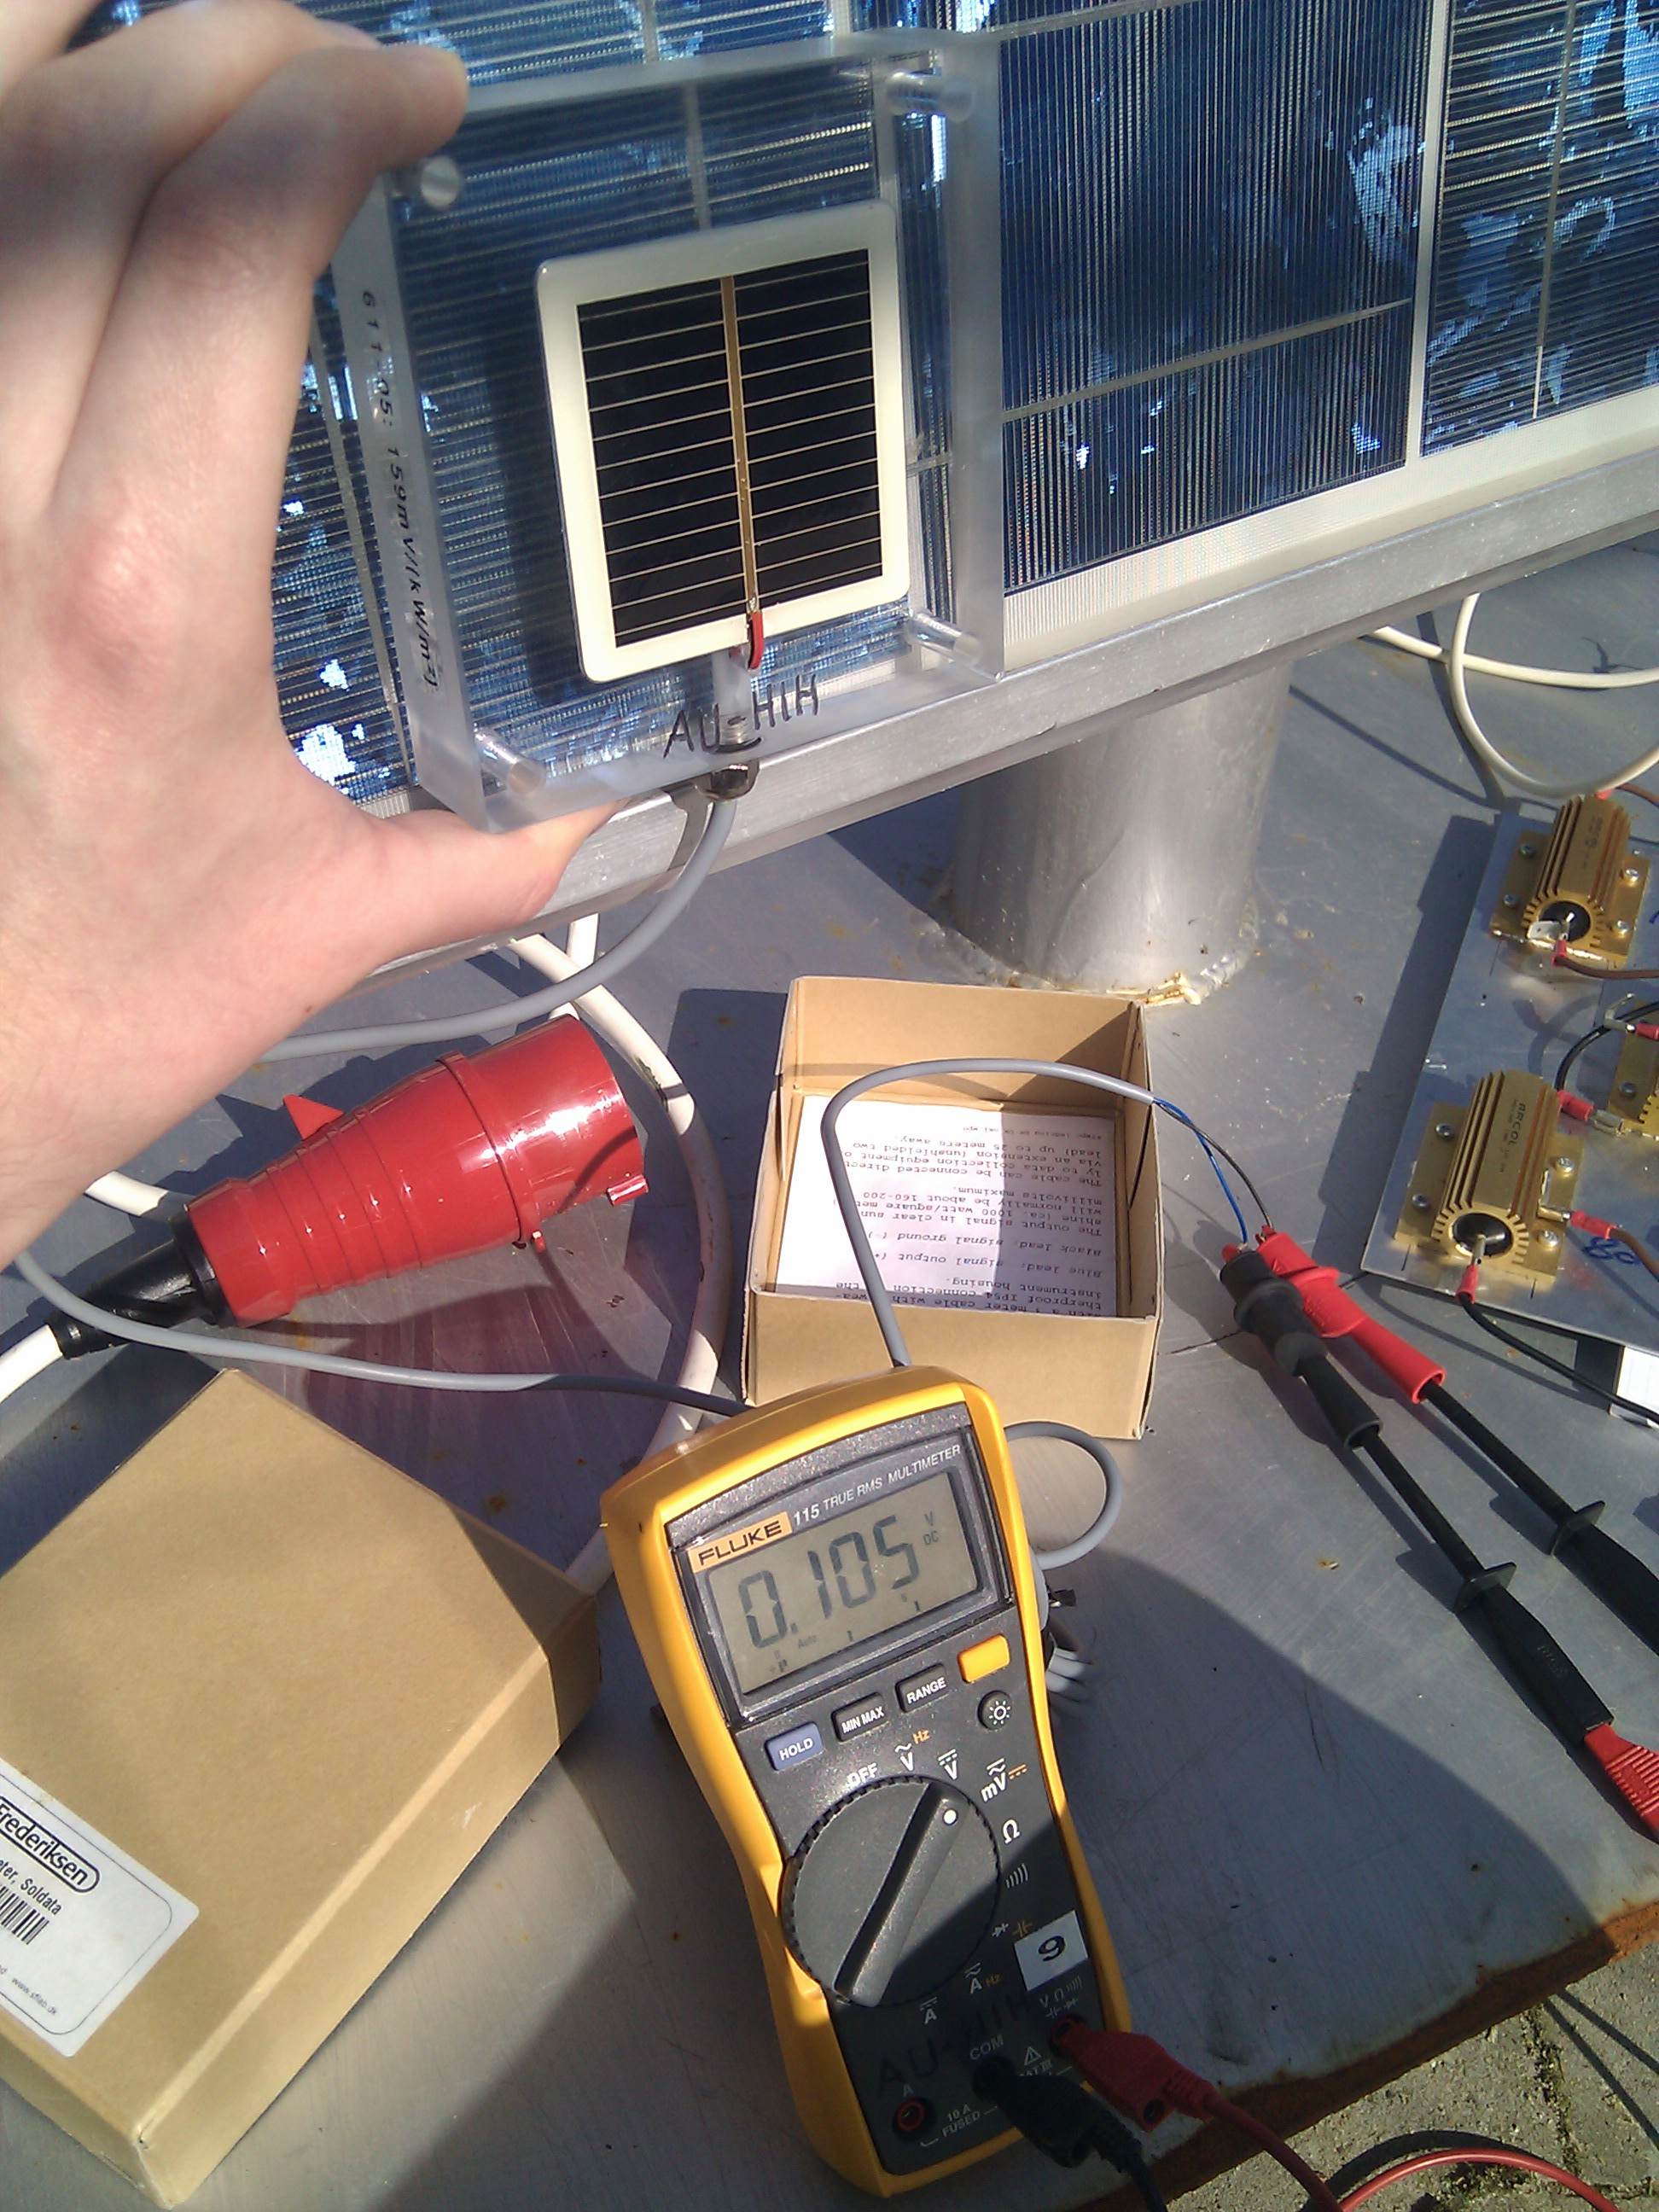
\includegraphics[width=5cm]{./img/sun_intensity}
\caption{Measuring of sun intensity}
\label{fig:sun_intensity}
\end{figure}

To find out how intense the sunlight was, a pyranometer was used. It was placed at the surface of the Photo voltaics, to measure at the same angle as the panel itself. This is shown at Figure \ref{fig:sun_intensity}. A multimeter was connected to the output, which measured 134mV. The pyranometer is calibrated to have a output of 159mV when the intensity equals $1000W/m^2$.\\
$134mV/(0.159mV/W)=842W/m^2$

\begin{figure}[H]
\centering
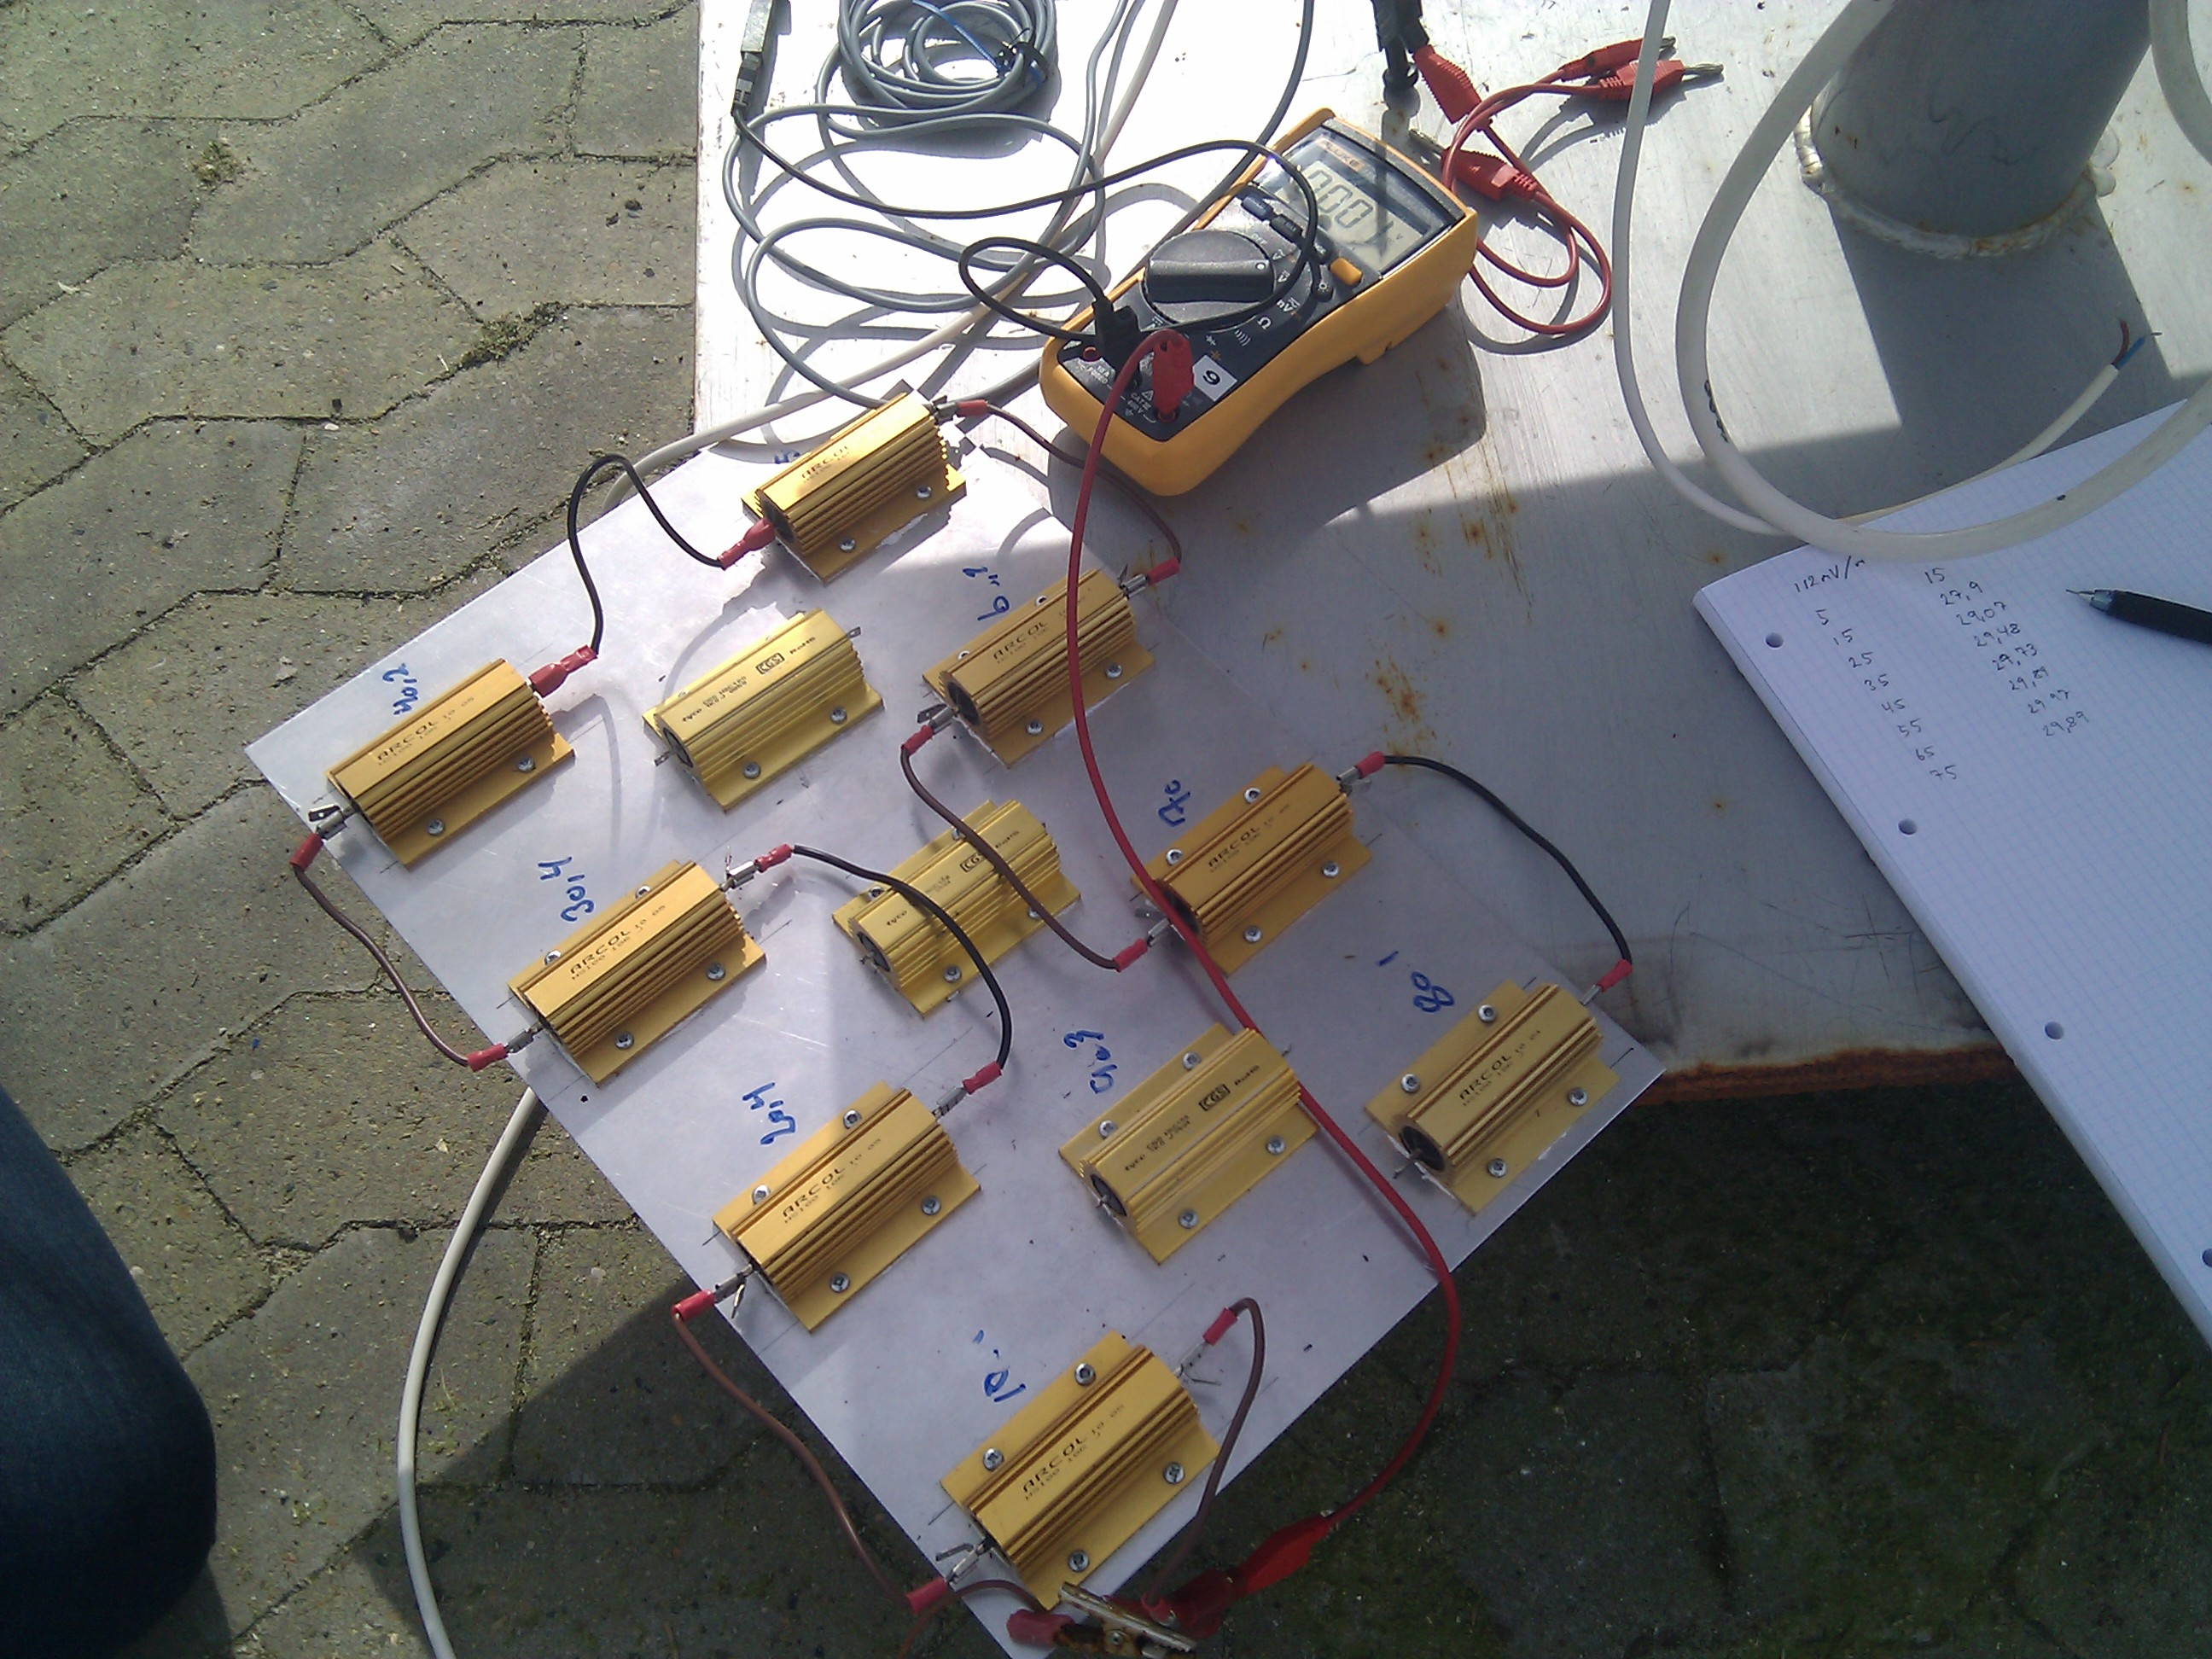
\includegraphics[width=6cm]{./img/IMG_20120326_140141}
\caption{Several resistors, to measure the effect of the Photo Voltaics}
\label{fig:IMG_20120326_140141}
\end{figure}


Now the output of the Photo Voltaic was measured. Only the output voltage was measured. It was measured across different resisstances, from 5ohms upto 125ohm, in steps of 5ohm. Then the current could be calculated from ohms law, and figures \ref{fig:Voltage_VS_Current-PV_effect} and \ref{fig:Voltage_VS_Power-PV_effect} shows the relation between load and power. \\


\begin{figure}[H]
\centering
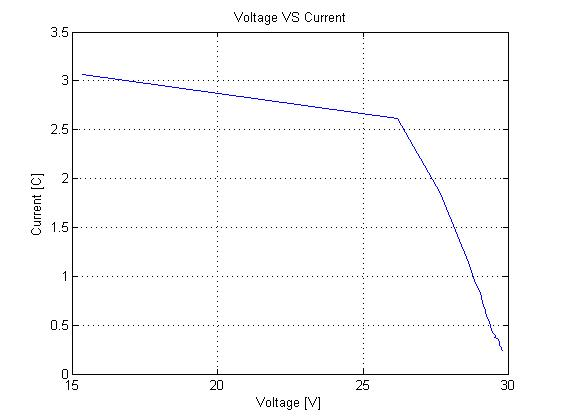
\includegraphics[width=8cm]{./img/Voltage_VS_Current-PV_effect}
\caption{Voltage VS Current - Photo Voltaics Effect}
\label{fig:Voltage_VS_Current-PV_effect}
\end{figure}

\begin{figure}[H]
\centering
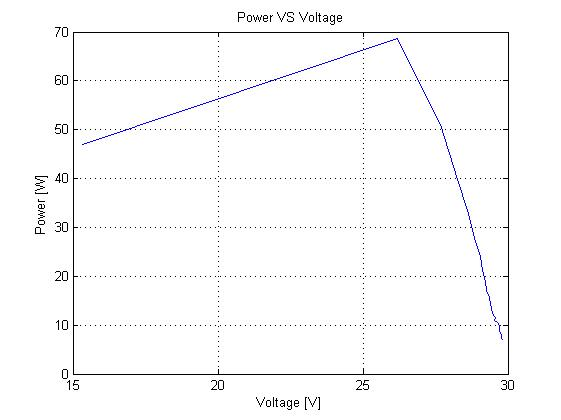
\includegraphics[width=8cm]{./img/Voltage_VS_Power-PV_effect}
\caption{Voltage VS Power - Photo Voltaics Effect}
\label{fig:Voltage_VS_Power-PV_effect}
\end{figure}

Its fund that the highest output effect is at almost 70watts. We also see that the Photo Voltaics has to be installed with the correct load, to give the highest power output. \\
This test was done on a sunny day, but not the MOST sunny day of all time. It is still unknown what the highest power output of the panel is, and it is hard to find out. \\

Other information about the panel may help, namely the open circuit voltage, measured at the output of the photo voltaics, without any load. The output was measured to 30.4V. \\
A lot of datasheets was inspected, in order to find matching photo voltaics, with the same characteristics of minimum 70W and a open circuit voltage of 30V. This voltage will not increase if the sun intensity increases, only the amperes will. This is the maximum voltage output, so that has to be fulfilled in the datasheet. The one matching the best, was from gernam solar power; GSP-P50-185. \hilight{\textbf{[DATASHEET]}} \\
The important properties that was compared:\\

\begin{tabular}{|l|l|l|}
\hline  & Data & Datasheet \\ 
\hline Open-circuit voltage Voc & 30.4V & 30.65V \\ 
\hline Rated voltage Vmpp & 70W & 185Wp \\ 
\hline 
\end{tabular} 

The open circuit voltage is very close to the target, but the watt-peak is not that close. The Watt-peak is measured in labs,m by applying $1000W/m^2$ to the Photovoltaics panel, and then measure the output across different resistances. Fortunately such a strong light is not available for us to use, but in the test made, the power was at $842W/m^2$. Another error is the "big" step in resistance. The rated voltage (Vmpp) of the target panel is at 25.05V. In the test made, a voltage was measured to 15.32V and 26.19V at 5 and 10 ohm resistance respectively. A resistance of lets say 8ohm may have lifted the watt-peak a bit. With these twop ewrrors in mid, the lack of $watt/m^2$ and the unprecise resistance may have decreased the performance of the panel. In order to the project work to contunie, this datasheet will be used, to find the highest voltage and current output of the photovoltaics. \\

Another important thing about these results, is that we doint need any galvanic isolation in the system. 30V and 8A is not enough to damage and/or disturb the PCBs, more than the problems it provokes can be solved in other, more cheaper and easier ways. 







\subsubsection{Design circuit for Log Module (Jacob)}
\paragraph{Requirements to fulfil}\mbox{}\\
FR.1.d\\
NR.1.a\\
None of the requirements will be completely fulfilled in this timebox, but during this period both should be kept in mind. 
\paragraph{Theory}\mbox{}\\

\begin{landscape}
\begin{figure}[H]
\centering
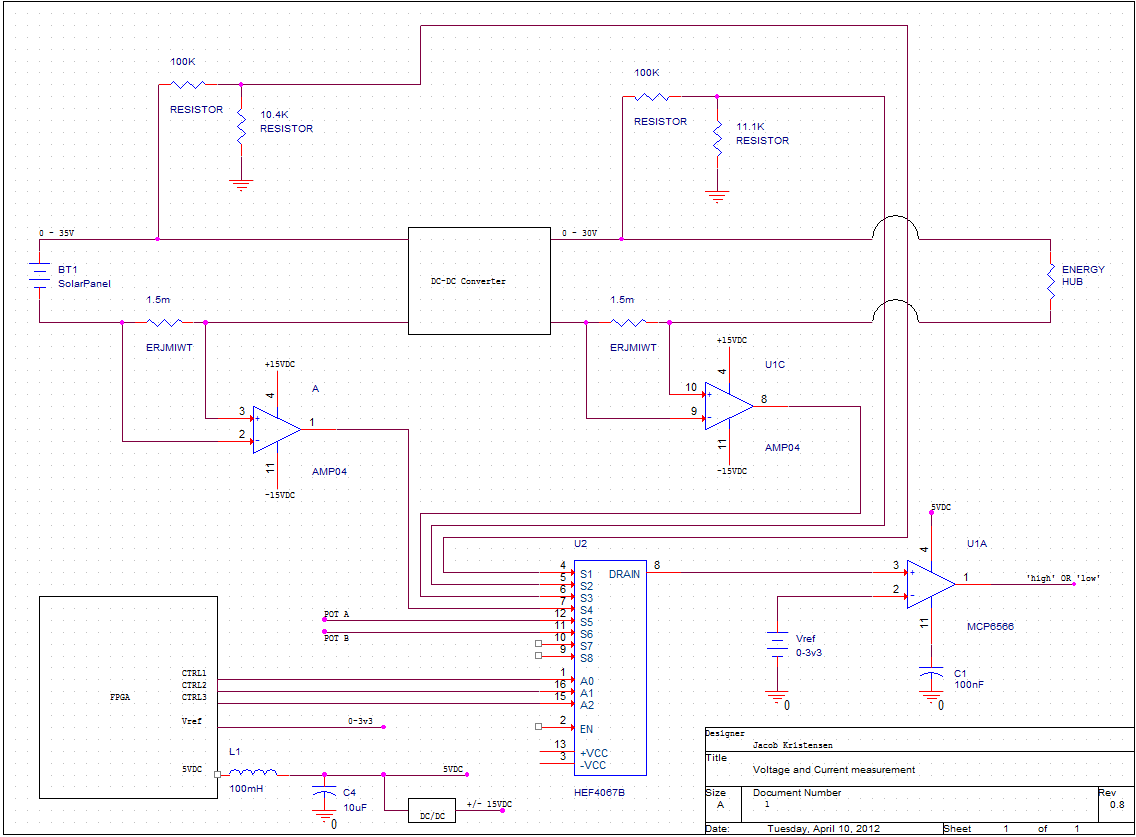
\includegraphics[width=20cm]{./img/vc_measure_schematic}
\caption{}
\label{fig:vc_measure_schematic}
\end{figure}
\end{landscape}

A schematic of the voltage/current measurement hardware is made, which is shown in figure \ref{fig:vc_measure_schematic}.\\
Leftmost a battery is placed, symbol of the Photo Voltaic. The maximum output has bin set to 35V, which is higher than the datasheet documents, but this is just to be sure. A PWM signal is used to compare the voltage, and not a R-ladder, which makes the steps smaller, and the measurement more precise. At the center the DC/DC converter is placed as a square. To the right a resistor is placed, symbol of the load (Energy Hub).\\
The voltage and the current has to be measured both before and after the DC/DC conversion. This gives two almost identical circuits on both sides of the DC/DC converter.\\
On top two voltage dividers is placed, to divide the voltage down to 3v3, which is the maximum input the FPGA can measure. A high input impedance of 100K ohm will ensure less loss in the circuit. \\
The equations to find the resistor values for the voltage dividers:\\
\begin{equation}
V_o=\frac{R_2}{R_1+R_2}*V_i
\end{equation}
\begin{equation}
3.3V=\frac{R_2}{100,000R+R_2}*35V
\end{equation}
\begin{center}
$R_2=10.4K ohm$
\end{center}

and now after the DC/DC, where the voltage must be at maximum 33VDC.
\begin{equation}
3.3V=\frac{R_2}{100,000R+R_2}*33V
\end{equation}
\begin{center}
$R_2=11.1K ohm$
\end{center}



Below the voltage dividers, two instrumental amplifiers (AMP04) are placed. They measure the voltage drop over a ERJMIWT (Power current measurement resistor), with an resistance of 1.5m ohm, which is very small, ensures as less loss in power as possible. These resistors are built for the purpose. \\
Also the instrumental amplifiers are optimized for measurements. They have a very low power consumption, they are very sensitive and does not get easily disturbed by interference from the surroundings, which makes them great for the purpose of measuring devices. \\
Both the outputs from the voltage dividers and from the amplifiers are sent to a multiplexer, which also receives the inputs from the pot-meters, measuring the position of the two motors turning the solar panel. They will be discussed later. The multiplexed signals will then be sent to a comperator (MCP6566), which receives a PWM reference input from the FPGA board. Then the FPGA can measure both current and voltage of input and output of the DC/DC converter. The multiplexer needs 3 signals to be controlled. \\
The instrumental amplifiers needs -+15VDC supply, which can be obtained by converting 5VDC into +-15VDC. This can be done by a converter from xppower.com. The 5VDC supply is placed on the FPGA board. This source can be very unstable, so in order to make it more stable, an LC circuit is placed at this output. This LC circuit consists of an inductor (L) and a capacitor(C). \\
To minimize the effect of fast-edges, and to decouple any track inductance, a de-coupling capacitor is added to the supply of the comparator. The capacitor should be placed as close to the amplifier as possible. Even though this will not be a big PCB, and thereby the track inductance wont be that big, it will not harm to place a 100mF capacitor at the supply. 


\paragraph{verification of requirements}\mbox{}\\




\end{document}


\end{document}
